\chapter{Methodology}
\label{sec:Methodology}
This chapter will present the whole procedure of the implemented anaphora resolution system with all of its stages. The complete system can also be examined online.\footnote{The download is available at https://github.com/HenryvanderVegte/henryvdv.BA}

\section{Preprocessing}
\label{preprocessingSection}
\begin{figure}[h]
	\centering

	\fbox{ \scalebox{0.96}{
  		\includegraphics[width=\linewidth]{figures/nlppipelinev5.pdf}
	}}
	\caption{Natural language preprocessing pipeline}
	\label{figure:nlppipeline}
\end{figure}

First of all, the required information of the training corpus needs to be extracted. The natural language preprocessing pipeline shown in Table \ref{figure:nlppipeline} was used.  The WikiCoref annotation scheme already includes information on tokens, sentences, and coreferential chains and could easily be extracted.

Still, several other information is missing in order to apply feature values (for instance, information on nominal phrases and part of speech). The \textit{Stanford CoreNLP} toolset \citep{manning-EtAl:2014:P14-5} was used to gain this information. More precisely, its part-of-speech tagger, named entity recognizer, and parser were applied. 
A part-of-speech tagger annotates for each token a word class. Word classes are, for instance, nouns or verbs. Additionally, the tagger differentiates also on more specific details like number or tense. In total, the tagset contains 52 different tags (the whole tagset is shown in Appendix \ref{table:AllPOSTags}). Note that the assigned labels for the part-of-speech tagger and the parser are simplified in the following examples in order to reduce its complexity. For instance, the implemented part-of-speech tagger will differentiate between singular and plural nouns while only the tag \textit{noun} is used in the examples.\\
The named entity recognizer identifies amongst other entities persons, organizations, and dates. \\
An illustrative example of these elements is shown in Figure \ref{figure:nlppipelineexample}. 

\begin{figure}[h]
	\centering
	\fbox{ \scalebox{0.96}{
  		\includegraphics[width=\linewidth]{figures/pipelineExample6.pdf}
	}}
	\caption{Annotation example}
	\label{figure:nlppipelineexample}
\end{figure}

The Parser can be subdivided into two different modules named constituent parser and dependency parser. 

The constituent parser divides the sentence into sub-phrases in a hierarchical order. The type of the phrase is defined by the central word in it (also called head word) \citep{jurafsky2014speech}. For instance, if the head word is a noun, the considered phrase is called noun-phrase. The most common kind of illustration is through a dependency parsed tree as shown in Figure \ref{figure:constituencytree}.

It should be noted that the level of granularity of the used tags is reduced in Figure \ref{figure:constituencytree} and Figure \ref{figure:dependencytree} in order to keep them as comprehensible as possible and to facilitate the start with parsed syntax trees. For instance, the dependency tag ``subject"  (abbreviated ``subj.") is normally subdivided into clausal subject, clausal passive subject, nominal subject, and nominal passive subject. Constituency parsed trees considered later in this work will also use abbreviations, whereas the tags in Figure \ref{figure:constituencytree} are written out. A whole list of all used constituency tags is given in Appendix \ref{table:AllConstituencyTags} and of all used dependency tags in Appendix \ref{table:AllDependencyTags}.

\begin{figure}[h]
	\centering
	\fbox{ \scalebox{0.96}{
  		\includegraphics[width=\linewidth]{figures/constituencyTree4.pdf}
	}}
	\caption{Simplified constituency parsed tree }
	\label{figure:constituencytree}
\end{figure}



The dependency parser describes the relationship of words among each other. A word that depends on another is linked to it. Additionally, the relationship between both words is annotated. Most graphic representations visualize the relationship through pointed arrows based on the governing word. An exemplary dependency parsed model is shown in Figure \ref{figure:dependencytree}. The arrow description will thereby represent the type of the relationship. The abbreviations subj., mod., obj., and det. represent subjects, modifiers, object, and determiners.


\begin{figure}[h]
	\centering
	\fbox{
	\scalebox{1.7}{ 
\begin{dependency}[theme = simple,label style={font=\sffamily,thick}]
   \begin{deptext}[column sep=1em]
 	 \textsf{John} \& \textsf{saw}  \& \textsf{her}  \& \textsf{at}  \& \textsf{the}  \& \textsf{park}  \\
   \end{deptext}
   \deproot{2}{root}
   \depedge{2}{1}{subj.}
   \depedge[edge start x offset=-2pt]{2}{6}{mod.}
   \depedge{2}{3}{obj.}
   \depedge[arc angle=50]{6}{5}{det.}
   \depedge{6}{4}{case}
\end{dependency}
	}	
}
	\caption{Dependency parsed tree}
	\label{figure:dependencytree}
\end{figure}


Coreferential information in WikiCoref is stored through a joint identification number for each coreferring annotation and can therefore be easily extracted. The third-person pronominal anaphoras were extracted of the coreference chain as follows: For each pronoun in the current document, search for the preceding phrase of its coreference chain. The pronoun will be tagged as the anaphora and the preceding phrase as the antecedent. 

As soon as all relevant information is annotated, a training set needs to be created. In order to do so, the procedure used by \cite{soon2001machine} was adopted. As already stated in Section \ref{soon2001traininginstances}, all anaphoras and their respective antecedents form thereby positive feature vectors while all intermediate noun phrases form negative feature vectors with their corresponding anaphoras. For instance, a sequence of noun phrases A-B-C-D with A coreferring D and D as a pronoun is considered. In this case the pair (A,D) forms a positive instance while (C,D) and (B,D) form negative instances.\\
The idea of selecting that approach is as follows: A human would reject all intermediate noun phrases due to several indicators that exclude the candidate for some reason. In contrast, noun phrases earlier in the text than the antecedent could be legitimate candidates if the antecedent did not exist. In conclusion, a valid rejection of candidates preceding the antecedent is only possible if the antecedent is already detected. However, if the antecedent is already detected no further examination needs to be done. With the algorithm of \cite{soon2001machine}, 904 positive and 2846 negative feature vectors were created in total.

The anaphora set consists of 17 reflexives (herself, himself, themselves, itself), 379 nominatives (he, she, they), and 508 possessives (their, its, her, his). There are several ways of dealing with the pronoun \textit{it} as it could either be referential or pleonastic (like the \textit{it} in ``it is raining"). Previous pronoun resolution systems either decide to manually exclude pleonastic pronouns \citep{kennedy1996anaphora,bergsma2005automatic}, or to identify and filter them. The identification of pleonastic pronoun can be considered as a natural language processing task on its own with several different approaches, leading from machine learning \citep{boyd2005identifying} to rule-based systems \citep{lappin1994algorithm}.\\
As the number of occurrences of \textit{it} is not decisive, it will be neglected in this work.

%aussortierte Fälle

\section{Feature Set}
The whole feature set can be divided in four different categories. There are features that only affect the anaphora, features that only affect the antecedent, features that describe the relationship between both, and features that are related to gender information. A whole list of features is shown in Table \ref{table:wholefeatureset}. The features are mostly adopted by \cite{bergsma2005automatic}, however there are several different implementations especially concerning the gender features.

\begin{table}[p]
\centering
  \caption{Pronoun resolution feature set}
	\scalebox{0.9}{ 
  \begin{tabular}{| l |r | r |}

    \hline
    Feature Type & Feature & Description \\ \hline
\hline

	\multirow{4}{1.3cm}{Pronoun referred} & Masculine & If pronoun is masculine: 1, else: 0 \\ \cline{2-3}
 	& Feminine &  If pronoun is feminine: 1, else: 0 \\	\cline{2-3}
	& Neutral &  If pronoun is neutral: 1, else: 0 \\	\cline{2-3}
	 & Plural & If pronoun is plural: 1, else: 0 \\ \hline
	\hline
	\multirow{17}{1.3cm}{Antecedent referred} & Antecedent Frequency & Number of occurrences / 10.0 \\ \cline{2-3}
 	& Subject &  If antecedent contains subject: 1, else: 0 \\ \cline{2-3}
	& Object &   If antecedent contains object: 1, else: 0 \\	\cline{2-3}
	& Predicate &   If antecedent contains predicate: 1, else: 0 \\ \cline{2-3}
	& Head-Word Emphasis &  If antecedent parent is no noun: 1, else: 0 \\	\cline{2-3}
	& Definite & If antecedent has definite article: 1, else: 0 \\ \cline{2-3}	
	& Pronominal &  If antecedent contains pronoun: 1, else: 0 \\	\cline{2-3}
	& Conjunction &  If antecedent is not part of conjunction: 1, else: 0 \\	\cline{2-3}
	& Prenominal Modifier & If antecedent contains prenominal modifier: 1, else: 0 \\ \cline{2-3}
	& Organization & If antecedent contains organization: 1, else: 0 \\ \cline{2-3}
	& Person & If antecedent contains person: 1, else: 0 \\ \cline{2-3}
	& Time & If antecedent contains time units: 1, else: 0 \\ \cline{2-3}
	& Date & If antecedent contains date: 1, else: 0 \\ \cline{2-3}
	& Money & If antecedent contains monetary name: 1, else: 0 \\ \cline{2-3}
	& Number & If the antecedent contains a number: 1, else: 0 \\ \cline{2-3}
	& His/Her & If antecedents first word is his or her: 1, else: 0 \\ \cline{2-3}
	& He/His & If antecedents first word is he or his: 1, else: 0 \\  \hline
	\hline
	\multirow{9}{1.3cm}{Pronoun and antecedent referred} & Binding Theory & If binding principles B is satisfied: 1, else: 0 \\ \cline{2-3}
 	& Same Sentence &  If both are in the same sentence: 1, else: 0 \\	\cline{2-3}
	& Intra-Sentence Diff. &  Difference in sentences / 50.0 \\	\cline{2-3}
	& In Previous Sentence & If antecedent is in previous sentence: 1, else: 0 \\ \cline{2-3}
	& Inter-Sentence Diff. & Difference in tokens / 50.0\\ \cline{2-3}
	& Prepositional Parallel & If both depend on the same preposition: 1, else: 0 \\ \cline{2-3}
	& Quotation Situation & If both are in or out quotes: 1, else: 0 \\ \cline{2-3}
	& Singular Match & If both are singular: 1, else: 0 \\ \cline{2-3}
	& Plural Match & If both are plural: 1, else: 0 \\ \hline
	\hline
	\multirow{11}{1.3cm}{Gender referred} & Standard Gender Match & If gender is known and matches: 1, else: 0 \\ \cline{2-3}
 	& Standard Gender Mismatch &  If gender is known and mismatches: 1, else: 0 \\	\cline{2-3}
	& Pronoun Mismatch &  If both are pronouns and mismatch: 1, else: 0 \\	\cline{2-3}
	& Masculine Mean & Mean $\mu$ of masculine distribution \\ \cline{2-3}
	& Masculine Std. Deviation & Std. deviation $\sigma$ of masculine distribution \\ \cline{2-3}
	& Feminine Mean &  Mean $\mu$ of feminine distribution \\ \cline{2-3}
	& Feminine Std. Deviation & Std. deviation $\sigma$  of feminine distribution \\ \cline{2-3}
	& Neutral Mean &  Mean $\mu$ of neutral distribution \\ \cline{2-3}
	& Neutral Std. Deviation & Std. deviation $\sigma$  of neutral distribution \\ \cline{2-3}
	& Plural Mean &  Mean $\mu$ of plural distribution \\ \cline{2-3}
	& Plural Std. Deviation & Std. deviation $\sigma$  of plural distribution \\ \hline

  \end{tabular}
}
	\label{table:wholefeatureset}
\end{table}

\subsection{Pronoun Features}
As the list of resolved pronouns is limited, a simple rule for each feature determines the gender values (for instance, if the pronoun is whether ``he",``'his", or ``himself", it is considered being masculine). 

\subsection{Antecedent Features}
The antecedent frequency is one of the few not binarized features. It is especially useful on Wikipedia articles, as they mostly address only a small amount of entities which are described in particular. \\
The information on grammatical relations for subject, object, and predicate features is gained through the dependency relationship of the covered words in the antecedent (Figure  \ref{figure:dependencytree}).\\
In order to get the Head-Word Emphasis feature value, the head noun needs to be identified (for instance, in the head noun of the phrase ``the park" is ``park" in Figure \ref{figure:constituencytree}). In a second step, the part-of-speech tags were used to check if the parent word is a noun.\\
Information on definite articles, pronouns, and conjunctions can also be observed through the part-of-speech tags.
The prenominal modifier value is observed through dependencies (an example for a modifier is also in Figure \ref{figure:dependencytree}) and the part-of-speech tag of its governing word. 
The features from organization to number are derived through the named entity values of the named entity recognizer module (Figure \ref{figure:nlppipeline}).
The last two features in this category are implemented through simple comparisons.

\subsection{Pronoun-Antecedent Features}
The most complex feature might be the binding theory implementation and needs therefore further explanation. The used principles of binding theory were formulated by \cite{chomsky1993lectures}. Principle A of binding theory is that an anaphora must be bound by an antecedent. Since the implemented pronoun resolution is based on that assumption, it does not need to be verified. In order to explain Principle B, three sentences will be considered:

\begin{center}
	\begin{enumerate}[label={(\arabic*)}]
	\item  \label{example1} John saw him.
	\item  \label{example2} John's father saw him.
	\item  \label{example3} John thinks that Peter saw him.
	\end{enumerate}
\end{center}

In \ref{example1} it is obvious, that the pronoun ``him" cannot refer to John. Unlike that, \ref{example2} and \ref{example3} do not have that restriction. However, in \ref{example2} the pronoun cannot refer to ``John's father". A simplified explanatory approach would be, that ``John" in \ref{example1} and ``John's father" in \ref{example2} are not deep enough in the sentence structure to appear as antecedent. Therefore, the constituency trees of the sentences will be considered. Note that in the following visualizations (Figure \ref{fig:twoTreeExample}) the framed words represent the phrase or sentence level, while the not framed represent the part-of-speech tags. S stands for Sentence, NP for noun phrase, and VP for Verb Phrase. On part-of-speech level, NN means noun, VB verb, PR pronoun, and POS for a possessive ending. 

\begin{figure}[h]
    \centering\sffamily
\fbox{
    \subfloat[Sentence \ref{example1}]{
\fbox{ \scalebox{1.2}{
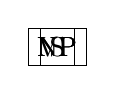
\begin{tikzpicture}
\tikzset{frontier/.style={distance from root=120pt}}
\Tree
 [.\node[draw]{S};
	[.\node[draw]{NP};
		[.NN John ]
	 ]
	[.\node[draw]{VP};
		[.VB saw ]
		[.\node[draw]{NP};
			[.PR him ]
		 ]
	 ]
 ]

\end{tikzpicture}
}
}
}%
    \qquad
    \subfloat[Sentence \ref{example2}]{
\fbox{ \scalebox{1.2}{
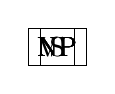
\begin{tikzpicture}
\tikzset{frontier/.style={distance from root=120pt}}
\Tree
 [.\node[draw]{S};
	[.\node[draw]{NP};
		[.\node[draw]{NP};
			[.NN John ] [.POS 's ]
		]
		[.\node[draw]{NP};
			[.NN father ]
		]
	 ]
	[.\node[draw]{VP}; 
		[.VB saw ]
		[.\node[draw]{NP};	
			[.PR him ]
		 ]
	 ]
 ] 
\end{tikzpicture}
}
}

}
}
    \caption{Constituency parsed examples 1 and 2}%
    \label{fig:twoTreeExample}%
\end{figure}

As it can be seen in Figure \ref{fig:twoTreeExample}, ``John" is deeper buried in the sentence structure in \ref{example2} than in \ref{example1}. This relationship can be expressed through c-commands. Its definition is: ''$\alpha$ c-commands $\beta$ if every node dominating $\alpha$ dominates $\beta$."\footnote{http://web.mit.edu/norvin/www/24.902/binding.html} In \ref{example1} the node ``John" c-commands the node ''him", but not in \ref{example2}. A first idea would be that a phrase that c-commands the anaphora cannot be the antecedent. That works for the first two sentences, but fails in the third one (Figure \ref{fig:ExampleTreeThree}). The new Tags are SB for subordinating clauses with an introduction, S' for subordinating clauses, and IN for prepositions.

\begin{figure}[h]
    \centering\sffamily
\fbox{ 

\begin{tikzpicture}
	\tikzset{frontier/.style={distance from root=200pt}}
	\tikzset{level 1+/.style={sibling distance=20pt}}
	\Tree   [.\node[draw]{S};
    [.\node[draw]{NP}; [.NN John ] ]
    [.\node[draw]{VP}; [.VB thinks ]
      [.\node[draw]{SB}; [.IN that ]
        [.\node[draw]{S'};
          [.\node[draw]{NP}; [.NN peter ]]
          [.\node[draw]{VP}; [.VB saw ]
            [.\node[draw]{NP}; [.PR him ] ] ] ] ] ] ]
	\end{tikzpicture}
}
    \caption{Constituency parsed example 3}%
    \label{fig:ExampleTreeThree}%
\end{figure}

In this case ``John" c-commands ``him", but appears as a possible candidate. As the subordinating clause seems to have an impact on the c-command rules, another limitation called binding domain needs to be considered. The binding domain determines the parts of the sentence in which a candidate can be excluded if it c-commands the anaphora. The binding domain is either defined as the smallest clause containing the anaphora, or the smallest clause containing the anaphora and a noun phrase that c-commands the anaphora. The former definition is chosen if the anaphora is the subject of a clause. 

Finally, Principle B can be defined as: An antecedent candidate can be excluded if it c-commands the anaphora and if it is located in its binding domain.

Principle C defines the handling of R-expressions. Those are noun phrases that are neither anaphoras nor pronouns \citep{crystal2011dictionary}. For instance, names fall into that category. An example of an r-expression would be the ``John" in ``He saw John". ``He" and ``John" cannot corefer, even though principle B is satisfied. Therefore, Principle C is defined as: ``R-expressions must be free" \citep{chomsky1993lectures}, or formulated differently: A corefering phrase is not allowed to c-command the r-expression. Principle C was implemented in this work, even though it might make a great difference as no cataphoras are detected by the implemented system.\footnote{Cataphoras are cases in which the referring noun stands is further in the text than its pronoun. For instance, in ``When he saw him, John smiled" \citep[p. 10]{cutting2005pragmatics}}

The next features that need further explanation are the singular and plural match implementations. The information on whether the pronoun is singular or plural is gained easily as the pronoun is considered as plural if it is ``their",``they", or ``themselves". The information on the antecedent is gained through its part-of-speech tag, as the used tags (Appendix \ref{table:AllPOSTags}) contain information on singular or plural.

\subsection{Gender Features}
The standard gender match or mismatch is detected through explicit surface clues. A noun phrase is considered as male or female if it contains a gender indicating designator like ``Mr." or ``Mrs.". A list of English honorifics was used to find those.\footnote{The used list is available at: http://self.gutenberg.org/articles/English\_honorifics} A second surface hint on gender agreement is if both are or contain pronouns of the same category (masculine, feminine, neutral, or plural).
Finally, corpus mined gender frequencies were assigned. The procedure is similar to the in Section \ref{section:gendercorpus} described approach of \cite{bergsma2005automatic} but with the corpus frequencies presented by \cite{Bergsma:06}. For instance, the $\alpha$ value for a masculine distribution would be the count of all masculine occurrences of the noun plus one and its $\beta$ would be the count of all times the noun occurred with any other gender plus one. The mean and standard deviation values are calculated as it is decribed in Section \ref{section:gendercorpus}.

\section{Baseline Approach}
The implemented baseline system detects always the previous noun phrase as the correct antecedent. Similar anaphora resolution systems also used this technique \citep{poesio2004general,bergsma2005automatic}.

\section{Machine learning-based Classifiers}
Several Support Vector Machine (SVM) classifiers were built in order to determine the influence of specific features or groups. The used implementation is SVM\textsuperscript{light} with a linear kernel \citep{joachims1999svmlight}. The anaphora resolution algorithm operates as follows: for each anaphora, the preceding noun phrases will be searched successively, beginning with the nearest. If no accepted noun phrase is found in the current and the previous sentence, the algorithm will terminate and assign a False Negative (FN) value for this anaphora. This means, that the algorithm assumes that the correct antecedent was falsely identified as wrong and therefore missed. This approach is different to \cite{bergsma2005automatic}, as it does not lower the threshold for acceptance until a matching antecedent is found. Even though the implementation of \cite{bergsma2005automatic} will increase the accuracy of the system (because the correct antecedent can be found in the initially neglected candidates while the implementation in this work cannot find those), it might distort the results. The pronoun resolution should rather aim for finding the correct antecedent in the regarded candidates.\\
 The chosen sentence distance is motivated by a look in the data. Approximately 97.4 \% of all considered antecedents could be found in the same or previous sentence of the anaphora.